\section{Programmation système : Multiprocessing}
\textbf{Warning: } Pour cette exercice, il a fallu reconfigurer le noyau linux en activant certaines options. Pour cela, se référer à la slide 72 du support de cours. Cette opération prend un temps considérable.
\subsection{Processus, signaux et communication}
\subsubsection{Exercice 1}
\textbf{Donnée:} Concevez	et	développez	une	petite	application	mettant	en	œuvre	un	des	services	de	communication
proposé	par	Linux	(p.ex.	« socketpair ») entre	un	processus	parent	et	un	processus	enfant.	
Le	processus	enfant	devra	émettre	quelques	messages	sous	forme	de	texte	vers	le	processus	parent,	
lequel	les	affichera	sur	la	console.	Le	message	« exit »	permettra	de	terminer	l’application.
Cette	application	devra	impérativement	capturer	tous	les	signaux	et	les	ignorer.	Seul	un	message	
d’information	sera	affiché	sur	la	console.\\\\
\textbf{Emplacement du code : } \textit{/Multiprocessing/Exercice1-Comm}\\

\textbf{Exécution du code : } \\
\begin{lstlisting}
lmi@csel1:~$ cd workspace/csel1/environment/multiproc/exercice1
lmi@csel1:~/workspace/csel1/environment/multiproc/exercice1$ make clean all
\end{lstlisting}

\begin{lstlisting}
# cd /usr/workspace/csel1/environment/multiproc/exercice1/                      
# ./app_a                                                                       
In the main process.                                                            

In the parent process                                                           

In the children process.                                                        

Enter a msg to send to the parent :                                             
Hello                                                                           
Hello will be written to the parent.                                            
Enter a msg to send to the parent :                                             
Received 50 from the children. String is : Hello                                
Bla                                                                             
Bla will be written to the parent.                                              
Enter a msg to send to the parent :                                             
Received 50 from the children. String is : Bla                                  
Received signal is : Interrupt                                                 
Received signal is : Interrupt                                                  
Bla will be written to the parent.                                              
Enter a msg to send to the parent :                                             
Received 50 from the children. String is : Bla                                  
Received signal is : Stopped                                                    
Received signal is : Stopped                                                    
Bla will be written to the parent.                                              
Enter a msg to send to the parent :                                             
Received 50 from the children. String is : Bla                                  
exit                                                                          
exit will be written to the parent.                                             
Received 50 from the children. String is : exit 
#
\end{lstlisting}

\subsection{CGroups}
\subsubsection{Exercice 2}
\textbf{Donnée:} Concevez	une	petite	application	permettant	de	valider	la	capacité	des	groupes	de	contrôle	de	limiter	
l’utilisation	de	la mémoire.	\\\\

\textbf{Emplacement du code : } \textit{/Multiprocessing/}\\

\textbf{Exécution du code : } \\
\begin{lstlisting}

\end{lstlisting}

\textbf{Réponse aux questions :}\\\\
\textbf{a. Quel	effet	a	la	commande	 « echo \$\$ > … »	sur	les	cgroups ?}\\
ee\\\\
\textbf{b. Quel	est	le	comportement	du	sous-système	« memory »	lorsque	le	quota	de	mémoire	est	
	épuisé ?	Pourrait-on	le	modifier ?	Si	oui,	comment ?}\\
ee\\\\
\textbf{c. Est-il	possible	de	surveiller/vérifier l’état	actuel	de	la	mémoire ?	Si	oui,	comment ?}\\
ee\\\\

\subsubsection{Exercice 3}
\textbf{Donnée:} Afin	valider	la	capacité	des	groupes	de	contrôle	de	limiter	l’utilisation	des	CPU,	concevez	une	petite	application	composée	au	minimum	de	2	processus	utilisant	le	100\%	des	ressources	du	processeur.	\\\\

\textbf{Emplacement du code : } \textit{/Multiprocessing/Exercice3-CPU}\\

\textbf{Monter les cgroup : } \\
\begin{lstlisting}
# mount -t tmpfs none /sys/fs/cgroup                                            
# mkdir /sys/fs/cgroup/memory                                                   
# mount -t cgroup -o memory memory /sys/fs/cgroup/memory                        
# mkdir /sys/fs/cgroup/memory/mem         
# mkdir /sys/fs/cgroup/cpuset                                                   
# mount -t cgroup -o cpu,cpuset cpuset /sys/fs/cgroup/cpuset                    
# mkdir /sys/fs/cgroup/cpuset/high         
# mkdir /sys/fs/cgroup/cpuset/low  
# echo 4 > /sys/fs/cgroup/cpuset/high/cpuset.cpus                               
# echo 0 > /sys/fs/cgroup/cpuset/high/cpuset.mems                               
# echo 3 > /sys/fs/cgroup/cpuset/low/cpuset.cpus                                
# echo 0 > /sys/fs/cgroup/cpuset/low/cpuset.mems                                 
\end{lstlisting}

\textbf{Réponse aux questions :}\\\\
\textbf{a. Les	4	dernières	lignes	sont	obligatoires	pour que	les	prochaines	commandes	fonctionnent	
	correctement. Pouvez-vous	en	donner	la	raison ?}\\\\
Les deux commandes écrivant dans le cpuset.cpus assignent un numéro de cœur pour le cpuset. Les autres écrivant dans le cpuset.mems limite l'espace mémoire et le crée. Cela crée l'architecture du CGroups. Pour l'avoir testé, si on n'affecte pas un cpuset.mems, l'application n'a pas de place en mémoire.
\begin{lstlisting}
# echo $$ > /sys/fs/cgroup/cpuset/low/tasks
sh: write error: No space left on device
\end{lstlisting}

\textbf{b. Ouvrez	deux	shells	distincte	et	placez en	une	dans	le	cgroup	high	et	l’autre	dans	le	cgroup	low.\\	
	Lancez	ensuite	votre	application	dans	chacune	des	shells.\\
	Quel	devrait	être	le	bon	comportement ?	Pouvez-vous	le	vérifier ?}\\\\
Installation de l'application avec la connexion sérielle: \\
Oui, on peut le vérifier, les commandes sont visibles un peu plus loin. Le comportement attendu est une utilisation à 100\% des cœurs 3 et 4 (attribués lors de la création du CGroup) du processeur avec 50\% pour le parent et 50\% pour le parent. Pour l'instant, on n'a pas assigné de limitation dans l'utilisation du temps CPU.\\
\begin{lstlisting}
lmi@csel1:~$ sudo minicom
...
# echo $$ > /sys/fs/cgroup/cpuset/high/tasks                                    
# ./app_a                                                                       
In the main process.                                                            

In the parent process                                                           

In the children process.  
\end{lstlisting}
Installation de l'application avec la connexion ssh: \\
\begin{lstlisting}
lmi@csel1:~$ ssh root@192.168.0.11
# echo $$ > /sys/fs/cgroup/cpuset/low/tasks
# cd /usr/workspace/csel1/environment/multiproc/exercice3/
# echo $$ > /sys/fs/cgroup/cpuset/low/tasks    
# ./app_a 
In the main process.

In the parent process

In the children process.

\end{lstlisting}

L'utilisation du CPU peut être affichée avec la commande top en lançant l'application en arrière plan:\\
\begin{lstlisting}
# ./app_a &                                                                     
# In the main process.                                                          

In the parent process                                                           

In the children process.  

# top
\end{lstlisting}

\begin{figure}[H]
	\begin{center}
		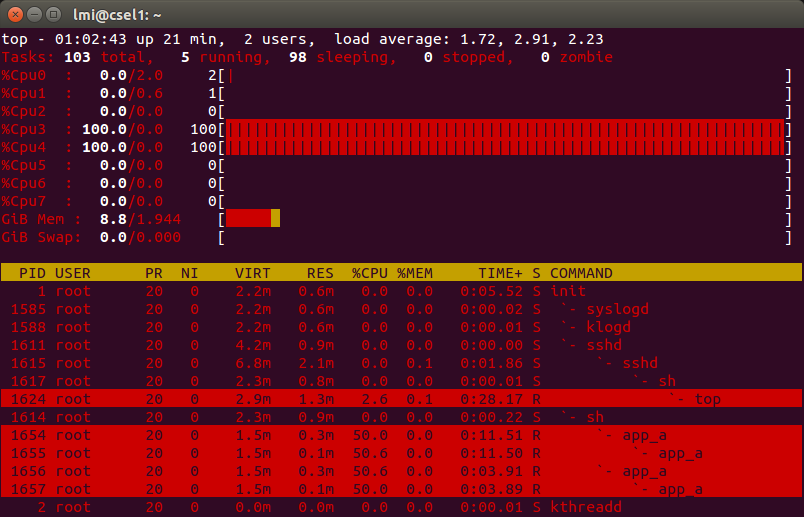
\includegraphics[width=16cm]{img/multiprocessCGroup.png}
		\caption{Utilisation du processeur}
		\label{multiprocess1}
	\end{center}
\end{figure}
\textbf{c. Sachant	que	l’attribut	cpus.shares permet	de	répartir	le	temps	CPU	entre	différents	
	cgroups,	comment devrait-on	procéder	pour	lancer deux	tâches	distinctes	sur	le	cœur	6	de	
	notre	processeur	et	attribuer	75\%	du	temps	CPU	à	la	première	tâche	et	25\%	à	la	deuxième ?}\\\\
Voici les commandes utilisées pour la configuration demandée. Par défaut, l'attribut cpu.shares contient 1024, qui représente 50\% du temps CPU. Pour plus de lisibilité, l'application a été compilée une fois sous le nom app\_a et une fois sous le nom app\_b.\\\\
Dans la connection ssh:
\begin{lstlisting}
# top
\end{lstlisting}
Dans la connection série:
\begin{lstlisting}
# echo 512 > /sys/fs/cgroup/cpuset/low/cpu.shares 
# echo 1536 > /sys/fs/cgroup/cpuset/high/cpu.shares  
# echo $$ > /sys/fs/cgroup/cpuset/low/tasks                                     
# ./app_b &                                                                     
# In the main process.                                                          

In the parent process                                                           

In the children process.                                                        

# echo $$ > /sys/fs/cgroup/cpuset/high/tasks                                    
# ./app_a &                                                                     
# In the main process.                                                          

In the parent process                                                           

In the children process.                                                        

# 
\end{lstlisting}
Voici le résultat obtenu, l'app\_a prend 75\% du temps CPU (37.7\% parent, 37.7\% enfant) et l'app\_b 25\%.
\begin{figure}[H]
	\begin{center}
		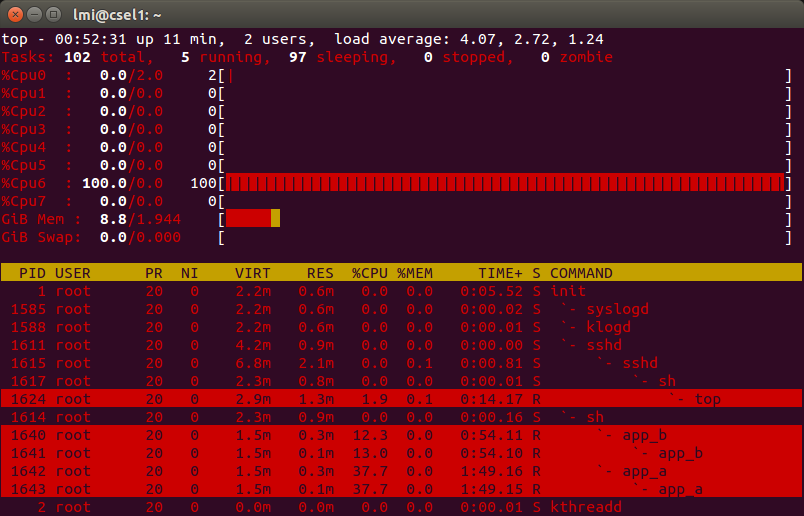
\includegraphics[width=16cm]{img/multiprocessCGroup2.png}
		\caption{Répartition du temps processeur}
		\label{multiprocess2}
	\end{center}
\end{figure}
